\documentclass[landscape,a4paper]{article}
\usepackage[utf8]{inputenc}
\usepackage[T1]{fontenc}
\usepackage{tikz}
\usetikzlibrary{shapes,positioning,arrows,fit,calc,graphs,graphs.standard}
\usepackage[nosf]{kpfonts}
\usepackage[t1]{sourcesanspro}
\usepackage{multicol}
\usepackage{wrapfig}
\usepackage[top=0mm,bottom=1mm,left=0mm,right=1mm]{geometry}
\usepackage[framemethod=tikz]{mdframed}
\usepackage{microtype}
\usepackage{mathpartir}

\usepackage{enumitem}% http://ctan.org/pkg/enumitem
\usepackage{amssymb} %% Definitions for math symbols.
\usepackage{amsmath} %% Definitions for math symbols.
\usepackage{enumitem}
\setlist{noitemsep, topsep=0pt,leftmargin=*}

\definecolor{myblue}{cmyk}{1,.72,0,.38}

\def\firstcircle{(0,0) circle (1.5cm)}
\def\secondcircle{(0:2cm) circle (1.5cm)}

\colorlet{circle edge}{myblue}
\colorlet{circle area}{myblue!5}

\tikzset{filled/.style={fill=circle area, draw=circle edge, thick},
    outline/.style={draw=circle edge, thick}}

\pgfdeclarelayer{background}
\pgfsetlayers{background,main}

\everymath\expandafter{\the\everymath \color{myblue}}
\everydisplay\expandafter{\the\everydisplay \color{myblue}}

\renewcommand{\baselinestretch}{.8}
\pagestyle{empty}

\global\mdfdefinestyle{header}{%
linecolor=gray,linewidth=1pt,%
leftmargin=0mm,rightmargin=0mm,skipbelow=0mm,skipabove=0mm,
}

\makeatletter % Author: https://tex.stackexchange.com/questions/218587/how-to-set-one-header-for-each-page-using-multicols
\renewcommand{\section}{\@startsection{section}{1}{0mm}%
                                {.2ex}%
                                {.2ex}%x
                                {\color{myblue}\sffamily\footnotesize\bfseries}}
\renewcommand{\subsection}{\@startsection{subsection}{1}{0mm}%
                                {.2ex}%
                                {.2ex}%x
                            {\color{red}\sffamily\bfseries}}
\makeatother
\setlength{\parindent}{0pt}

\begin{document}
\begin{multicols*}{3}
\fontsize{6pt}{5pt}\selectfont
% \section*{OS Basics}
\begin{description}
  \item[OS] Intermediary b/w user \& HW, executes user programs. convenience, control and coordinate HW  (efficiency).
  \item[OS Services] user interface; prog execution; I/O operations; file-system manipulation; communication between Ps; error detection; res alloc; accounting – who uses how much of what; protection and security
  \item[Direct Memory access] Allow I/O devices to transfer data directly to/from main mem without involving CPU. (1 Interrupt per Data block) %NOTE: instead of 1 per byte (cpu cache)
  \item[Interrupt] request for processor to interrupt current executing code. Processor suspends activities, saves its state and starts executing/gives control to \textbf{Interrupt Service Routine}. \textbf{Interrupt Vector}: contains addresses of all (interrupt) service routines. OS is interrupt driven.
  \item[Trap, Exception] Software-generated interrupt. Caused by software error, system call, other process problems.
  \item[OS data structures] OS needs Lists, stacks queues, trees, maps
\end{description}

\subsection*{Multiprocessor (MP) Systems}
\begin{description}
\item[Advantages]Increased Throughput, Economy of scale, Reliability
  \item[Generic Approach] Each processor performs all (types of) tasks. OS shared among CPUs, each CPU has local private copy of OS data structures.
  \item[Asymmetric MP] Each processor is assigned a special task. Master CPU runs OS, other Slave CPUs run user processes.
  \item[Symmetric MP] Each processor performs all (types of) tasks. OS shared among CPUs. (Lock on OS)
  \item[Non-Uniform Memory Access (NUMA)] Interconnected CPUs each with private mem. They logically share one physical mem space.
  \item[Clustered Systems] Like MP, but multiple computers working together. Linked via some kind of network %NOTE: (e.g LAN).
\end{description}

\subsection*{OS Operations}
\begin{description}
    \item[Bootstrap Program] Initializes system, loads OS kernel and starts execution at power-up. (Stored in \textit{Firmware}). \hfill Degree of Multiprog = Nr. of Ps in mem.
  \item[Batch System, Multiprog.] schedule jobs so CPU always has one job to execute (keep job queue in mem).
  \item[Timesharing, Multitasking]  fast switching between jobs. interactivity for user(s). illusion of concurrency
  \item[Dual-Mode]User/Kernel. Distinguish whether system is running user or kernel code with a HW provided \textbf{Mode bit}. privileged instructions only run in kernel mode; sys. call $\rightarrow$ kernel mode. return $\rightarrow$ user mode. %NOTE: Timer (prevent $\infty$)
\end{description}

% \section*{OS Structures}

\subsection*{System Calls}
\begin{description}
    \item[System Call] Programming Interface to services provided by the OS written in high-level lang (C or C++), below user interface.
   \item[System Call Interface] Each system call associated with a number, Sys. Call interface maintains a table of those numbers, calls OS to execute and returns status and output.
   \item[Parameter passing] Either by passing parameters into registers (limited); or store them in a memory block and pass addresses in a register (unlimited length of parameter, limited amount of parameters); or push them onto stack (unlimited amount \& length)
  \item[Syscall types] File management, Device management, Information management, Communications, Protection

\end{description}

\subsection*{System Programs}
\begin{description}
  \item[System Program]Provides convenient environment for program development and execution. Often they are user interfaces to system calls
  \item[System Program Types] File management, Status information, Programming-language support, Program loading and execution, Communications, Background Services (daemons)
\end{description}

\subsection*{Application Programs}
\begin{description}
  \item[Application Programs]  designed to carry out a specific task other than one relating to the operation of the computer itself, typically to be used by end-users, e.g. web browsers.
\end{description}

\subsection{Creation of processes}
\begin{description}
  \item[1. Preprocessing] Reads c file, processes includes, expands macros, handles conditional compilation.
  \item[2. Compilation] Produces object code (.o), i.e. sequences of bytes, loadable into any memory location
  \item[3. Linking] Combines all object and library files into one executable file. Solves unresolved external references. Relocates machine addresses
  \item[Dynamic Linking] Conditionally linked libraries. Loads system libraries only once.
  \item[Static Linking] Necessary library functions are embedded directly in exe.
  \item[4. Loading] Shell/click creates P, invokes loader, loads exe to RAM. OS allocates memory, relocates memory addresses.
  \item[5. Execution] Program is a running P, CPU starts processing, upon completion returns status, releases resources, removed from memory



  \item[Executables across OSs] Apps compiled on one OS are not executable on other OSs. (differing system calls, binary formats, instruction sets application binary interface). Can be solved via interpreted langs, virtual machines, use of standard API with compiler generating binaries in OS specific language (e.g. POSIX)

\end{description}

\subsection{OS Structures}
\begin{description}
  \item[Monolithic Systems]Includes everything between user prog and hardware. + fast kernel communication, + little overhead, + easy interaction between OS modules, - difficult to change, maintain, - single failure can cause system crash, - gets complex fast.

  \item[Loadable Kernel Modules] Kernel can load independent modules such as device drivers when needed. Like layered Modules but more flexible as kernel can communicate directly. (Linux has this)
  \item[Layered Module Structure] OS is divided into layers, each built on top of lower layers. Each layer implements service and communicates only to lower level layers.
    \item[Microkernel Systems] Everything in user mode, except scheduling, virt. mem. and basic IPC in kernel mode. + easy to extend, + more reliable and secure, + easier to port, - more performance overhead of kernel and user space communication.
      \item[Hybrid Systems] Combines microkernel and monolitic approach to address performance, security, usability needs. OS partially in kernel and user mode e.g. Linux
\end{description}

% \section*{Process Management}
\begin{description}
    \item[Process] Program loaded into mem, in execution.
  \item[Program] Passive entity stored on disk
  \item[Process states] new, ready, running, waiting, terminated
  \item[Process Control Block] Information about each P: P state, P number, PID, program counter, CPU registers, Mem.-management information (allocated mem for process), I/O status, CPU scheduling info (e.g. priority), Accounting info (e.g. CPU used)
  \item[Context Switch] When CPU switches to another P, save PCB of prev. P, load PCB of new P. (overhead)
\end{description}

\subsection*{Processes Layout}
\begin{tikzpicture}[remember picture,overlay]
    \node[xshift=76mm,yshift=5mm] at (current page.south west){%
    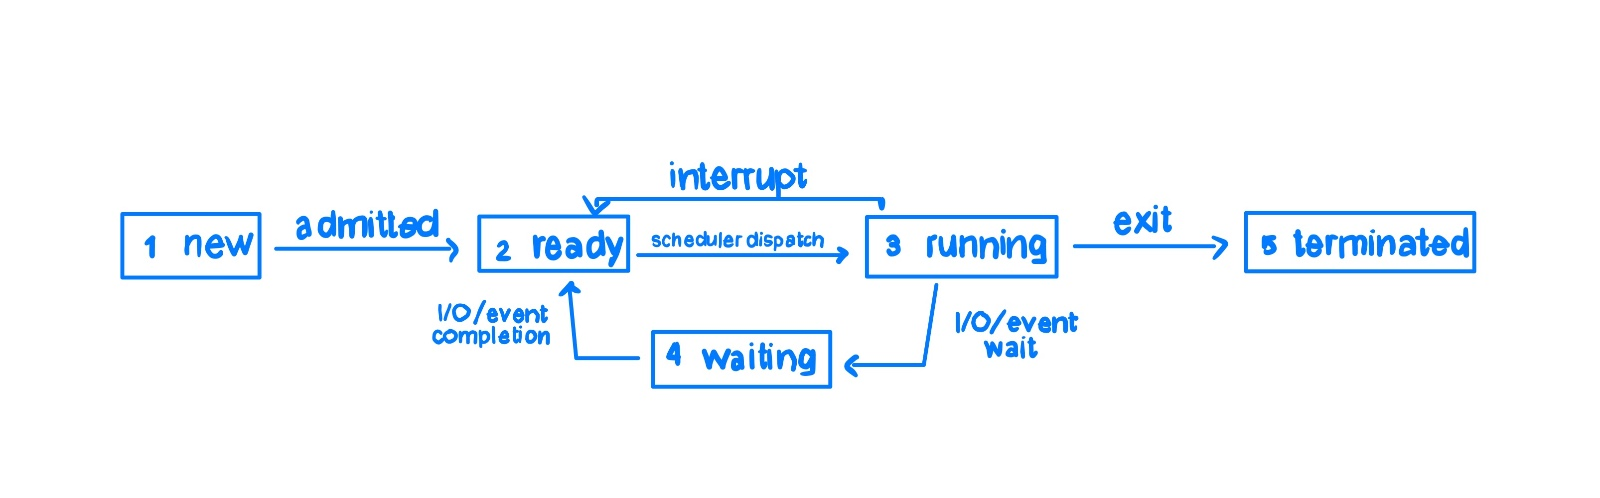
\includegraphics[width=55mm]{process_states.jpeg}};
\end{tikzpicture}
\begin{description}
  \item[Stack] temporary data: function parameters, return addresses, local variables
  \item[Heap] dynamically mem allocated during execution
  \item[data] Global variables
  \item[text] executable code
\end{description}

\subsection*{Operations on processes}
\begin{description}
  \item[Process creation]Parent P creates child (fork()) which can create own children → tree structure, every P has a unique identifier (PID). Either parent and child share all, a part or no resources.
  \item[Process termination] P's del themselves w/ exit(). Parent del child w/ abort(). Parent waits for child to end w/ wait(). child → \textbf{zombie} if child terminates before/w/o parent wait(), → \textbf{orphan} if parent terminates.
\end{description}

\subsection*{Interprocess communication}
\begin{description}
    \item[Cooperating P's](vs. Independent P's) execute concurrently, may be interrupted, share data. Need IPC
    \item[Shared Memory]Communication is under control of user P (not OS), P's share mem. space. Issue: \textbf{Producer-Consumer problem}: information to communicate stored in buffer. \textbf{unbounded:} no size limit, prod. can always produce, nice but unrealistic. \textbf{bounded:} fixed-size buffer. producer must wait if full.
  \item[Message passing] Communication controlled by OS, Messaging b/w P's w/out shared variables.\\
    \textbf{Communication Link}: \textit{Physical} (shared mem, HW bus, network). \textit{Logical}: direct/indirect, sync/async (blocking, non-blocking, rendez-vous),buffering (zero (sync r-v.)/bounded/unbounded capacity).
  \item[Direct Message passing] A link is established b/w P's. They must name each other explicitly (send(P,message), receive(Q,message)). Only one communication link. uni/bidirectional.
  \item[Indirect message passing] Messages are sent and received from mailboxes (i.e. ports). May share several communication links. uni/bidirectional.
  \item[Ordinary Pipe] Comm. b/w parent and child, cannot be accessed from outside the P that created it. Have a read end (fd[1]) and write end (fd[0]). Exists until P completion. (unidirectional)
  \item[Named Pipe, FIFO] Several P's can use pipe for communication. Exist until deleted. Appears as a file. (bidirectional: half/full duplex) %NOTE: duplex: travel one direction at the time or both at the same.
  \item[Socket] Endpoint of communication b/w machines, concatenation of IP and port. Data is sent via packets.
  \item[Remote Procedure Calls] abstract procedure (function) calls between Ps on networked systems. %NOTE: function can be invoked by P on another computer.
\end{description}

\section*{Synchronization}
Cooperating Processes execute concurrently, may be interrupted at any time and have access to shared data. Proper sequencing and coordination of processes is needed to maintain data consistency.
% access: LAS or shared memory/message passing
\subsection*{Race Conditions}
\begin{itemize}
    \item \textbf{Execution} outcome dependent on order of concurrent access to shared data
        \item \textbf{examples:} counter in prod-consumer-problem, PID
        \item \textbf{solutions:} disabling interrupts (single core vs. multiprocessors (time-consuming), affects system clock)
        \item \textbf{preemptive kernel}: process preempted in kernel mode, most common. more responsive, suitable for real-time programming
            % TODO: verstehen
    \item \textbf{non-preemptive kernel}: uncommon, process blocks CPU
\end{itemize}
\subsection*{Critical Section Problem}
\begin{itemize}
    \item \textbf{critical section} is where a process accesses shared data
    \item no two processes should be executing in their critical sections at the same time
    \item \textbf{solution:} mutual exclusion, progress (selection cannot be postponed indefinitely), bounded waiting (limit on waiting)
\end{itemize}
\begin{description}
    \item[Peterson's Solution] 2 processes, int turn, bool flag[2] shared, acquire \& lock, not guaranteed to work on modern computer architectures (requires atomic load/store, no instruction reordering)
    \item[Mutex Lock] acquire() and release() lock (atomic), bool available (binary), require busy waiting (spinlock, no context switch required)
    \item[Semaphores] integer variable, accesses through wait() and signal. busy wait \\
        - \textbf{counting} (init to nr of resources available, decr. in wait) vs. \textbf{binary} semaphore (like mutex lock). \\
        -  \textbf{implementation with suspension and waiting queues} %TODO:: S. 26ff
    \item[Monitors] high level form of process sync. \\
        - \textbf{condition variables} wait and signal on condition var.   \\
        - \textbf{mutex locks}
    \item[Priority Inversion] solution: \textbf{priority-inheritance protocol}: inherit higher priority until finished with resources %TODO: Definition  Priority Inversion
    \item[Deadlock]: 2 or more processes are waiting indefinitely for an event that can be caused only by one of the waiting processes.
\end{description}
\subsection*{Examples}
WEITER BEI S. 4 (04 - 2 Examples
\begin{description}
    \item[Bounded Buffer]
    \item[Dining Philosophers]
    \item[Synchronization within the Kernel]
    \item[POSIX Sync]
    \item[Alternative Approaches]
\end{description}
\subsection*{Deadlocks}
% starvation

%\vfill\null
%\columnbreak
\end{multicols*}
\end{document}
